% 方向导数

\pentry{全微分\upref{TDiff}, 点乘\upref{Dot}, 正交归一基\upref{OrNrB}}

先来看一幅等高线图(\autoref{DerDir_fig1}). 令高度 $z$ 为位置的函数$z = f(\vec r)$. 这里 $\vec r$ 是位矢\upref{Disp}, 即 $f(\vec r) = f(x,y)$. 当位矢沿着等高线移动时, $z$ 不变,而当位矢沿垂直于等高线的方向移动时, $z$ 变化得最快.位置沿其他方向运动, $z$ 的变化速度介于两者之间.

\begin{figure}[h]
\centering
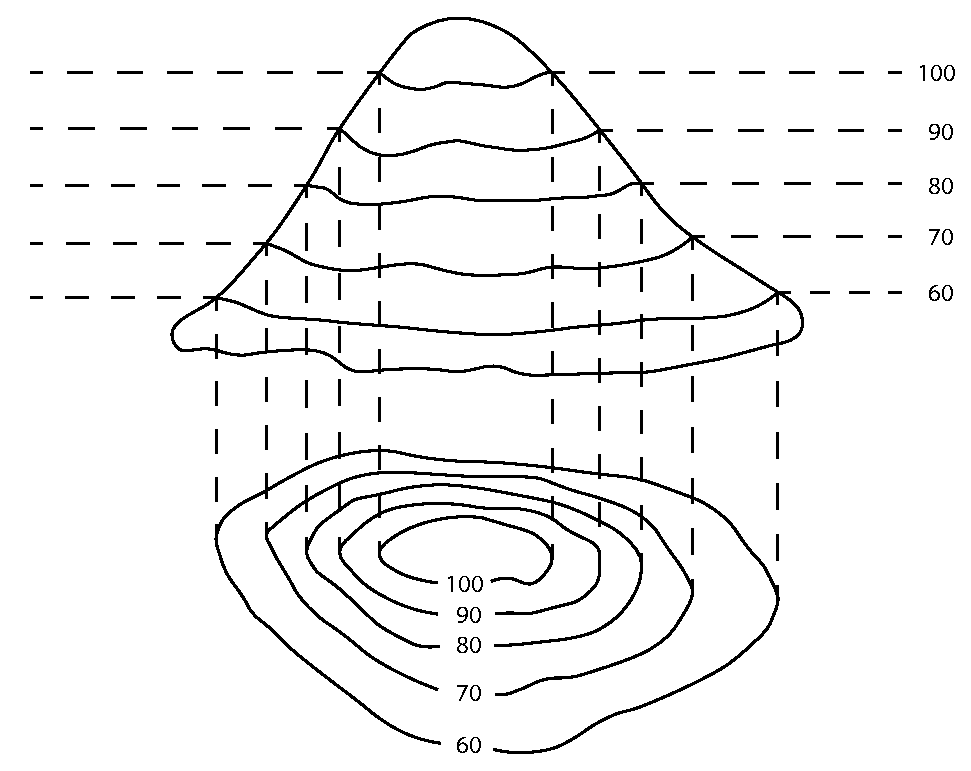
\includegraphics[width=9cm]{./figures/DerDir.pdf}
\caption{等高线}\label{DerDir_fig1}
\end{figure}

那么如何衡量位置向各个方向移动时 $z$ 变化的快慢呢? 我们先规定一个方向 $\uvec n = (n_x,n_y)$( 平面单位矢量,满足 $n_x^2 + n_y^2 = 1$), 然后用\textbf{方向导数}来衡量变化率,其定义如下
 \begin{equation}
\frac{{\D f}}{{\D n}} \equiv \mathop {\lim }\limits_{\Delta s \to 0} \frac{{f\left( {\vec r + \uvec n\Delta s} \right) - f\left( {\vec r} \right)}}{{\Delta s}} = \frac{{\D f}}{{\D s}}
\end{equation}
其中 $\uvec n\Delta s$ 代表沿 $\uvec n$ 方向的微小位移.从几何上来讲,二维函数 $f(\vec r)$ 表示一个曲面,曲面上某点的方向导数就是曲面在该方向的斜率.


% 以下的解释应该给全微分! 这里直接引用全微分的结论即可!
由“全微分\upref{TDiff}”中的结论
\begin{equation}
\D f = \pdv{f}{x} \D x + \pdv{f}{y}\D y
\end{equation}
而现在我们往 $\uvec n = \left( {{n_x},{n_y}} \right)$ 方向移动 $\D s$,所以
\begin{equation}
\D x = n_x \D s \qquad \D y = n_y \D s
\end{equation}
代入上式,得
\begin{equation}
\D f =  \left(\pdv{f}{x} n_x + \pdv{f}{y} n_y \right) \D s
\end{equation}
根据导数与微分的关系(也可以通俗地说“两边同除 $\D s$”), 就得到方向导数
\begin{equation}
\pdv{f}{n} = \dv{f}{s} = \pdv{f}{x} n_x + \pdv{f}{y} n_y
\end{equation}
如果使用平面的正交归一基\upref{OrNrB} $\uvec x, \uvec y$ 写成矢量点乘\upref{Dot} 的形式,就是
\begin{equation}
\frac{{\D f}}{{\D n}} = \left( {\frac{{\partial f}}{{\partial x}}\,\uvec x + \frac{{\partial f}}{{\partial y}}\,\uvec y} \right) \vdot \uvec n
\end{equation} 
定义\textbf{二维直角坐标系中的 Del 算符}为
\begin{equation}
\grad  = \uvec x\frac{\partial }{{\partial x}} + \uvec y\frac{\partial }{{\partial y}}
\end{equation}
其作用在函数上表示
\begin{equation}
\grad f = \frac{{\partial f}}{{\partial x}}\,\uvec x + \frac{{\partial f}}{{\partial y}}\,\uvec y
\end{equation} 
则方向导数可以写成相当简洁的形式,即
\begin{equation}\label{DerDir_eq7}
\frac{{\partial f}}{{\partial n}} = \grad f \vdot \uvec n
\end{equation} 

\subsection{多元函数的方向导数}
通过和以上类似的分析,可以得出 $N$ 元函数 $f(\vec r) = f(x_1,x_2\dots x_N)$ 在单位方向矢量 $\uvec n = \left( {{n_{x1}},{n_{x2}}\dots{n_{x_N}}} \right)$ 的方向上的微分关系为
\begin{equation}
\D f = \frac{{\partial f}}{{\partial {x_1}}}\D {x_1} + \frac{{\partial f}}{{\partial {x_2}}}\D {x_2}\ldots = \left( {\frac{{\partial f}}{{\partial {x_1}}}{n_{x1}} + \frac{{\partial f}}{{\partial {x_2}}}{n_{x2}}\dots} \right)\D s
\end{equation}
方向导数为
\begin{equation}
\frac{{\partial f}}{{\partial n}} = \frac{\D f}{\D s} = \left( {\frac{{\partial f}}{{\partial {x_1}}}{{\uvec x}_1} + \frac{{\partial f}}{{\partial {x_2}}}{{\uvec x}_2}\ldots  \frac{{\partial f}}{{\partial {x_N}}}{{\uvec x}_N}} \right) \vdot \uvec n = \grad f \vdot \uvec n
\end{equation} 
形式与\autoref{DerDir_eq7} 相同.这里定义了\textbf{ $N$ 维直角坐标系的 Del 算符} 为
\begin{equation}
\grad  = {\uvec x_1}\frac{{\partial f}}{{\partial {x_1}}} + {\uvec x_2}\frac{{\partial f}}{{\partial {x_2}}}\dots{\uvec x_n}\frac{{\partial f}}{{\partial {x_N}}} 
\end{equation}


